\documentclass[12pt,letter]{article}
\usepackage{../downey_format}

\begin{document}

	% set the section number, along with figure and equation numbers
	\setcounter{section}{2}	
	\setcounter{figure}{0}   
	\renewcommand\thefigure{\thesection.\arabic{figure}}
	\setcounter{equation}{\thesection}   
	\renewcommand\theequation{\thesection.\arabic{equation}}

	\section{Classification}

In Chapter~1, we examined various tasks that machine learning excels at, such as regression (predicting values) and classification (identifying classes). Having explored linear and polynomial regression in Chapter~2, we now turn our attention to classification in this section.







\subsection{Binary Classifier}

A binary classifier is a model that assigns inputs to one of two distinct classes.
Linear binary classification is a simple but powerful method used to separate data into two distinct classes by drawing a straight decision boundary---such as a line (in 2D) or hyperplane (in higher dimensions)---between them. It works by computing a weighted sum of the input features and applying a threshold to determine the output class. Mathematically, it learns a weight vector $\boldsymbol{\theta}$ and bias term $b$ such that the decision rule can be written as:
\begin{equation}
\hat{y} = \begin{cases}
1 & \text{if } \boldsymbol{\theta}^\text{T} \mathbf{x} + b \geq 0 \\
0 & \text{otherwise}
\end{cases}
\end{equation}
where $\mathbf{x}$ is the input feature vector. During training, the weights are adjusted to minimize classification error, often using gradient descent on a suitable loss functions (e.g., hinge loss or logistic loss). 

Despite its simplicity, the linear classifier is often surprisingly effective, especially when the data is linearly separable or nearly so. An example of such a case is shown in figure~\ref{fig:x_y_plot_linear_classifier} where the three models ($H_1$, $H_2$, and $H_3$) are linear models defined by the hyperparameters $ \boldsymbol{\theta}$ that each correctly classify the data. The challenge then becomes how does one obtain the hyperparameters $ \boldsymbol{\theta}$. To start, we will show that the hyperparameters $ \boldsymbol{\theta}$ can be obtained through gradient descent.



\begin{figure}[H]
    \centering
    \includegraphics[]{../figures/x_y_plot_linear_classifier}
    \caption{Linear classifier that can be implemented with gradient descent.}
    \label{fig:x_y_plot_linear_classifier}
\end{figure}


\begin{data}
\textbf{MNIST (Modified National Institute of Standards and Technology) Dataset}

\noindent  In this chapter, we utilize the MNIST (Modified National Institute of Standards and Technology) dataset, a collection of 70,000 small images of handwritten digits. This dataset is known as ``modified'' because it combines two earlier sets of images: one created by U.S. high school students and another by US Census Bureau employees. First published in 1998, the dataset is particularly suitable for machine learning tasks as each image is labeled with the digit it represents. Each digit has been normalized and centered in a 28x28 pixel frame and anti-aliased to introduce grayscale levels.

Typically, the dataset is split into two parts: the first 60,000 images are used for training, and the remaining 10,000 serve as validation data. It is standard practice to train and test models on the first 60,000 images, reserving the last 10,000 for final validation at the end of the project when the classifier is ready for deployment.

\begin{figure}[H]
    \centering
    \includegraphics[width=6.0in]{../figures/MNIST_data_set}
    \caption{A collection of the 10 digits (0-9) that make up the MNIST data set.}
    \label{fig:MNIST_data_set}
\end{figure}

Scikit-Learn includes a helper function that facilitates the downloading of the MNIST dataset.


\begin{figure}[H]
	\centering
	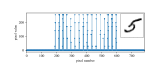
\includegraphics[width=6.0in]{../figures/MNIST_digit_features}
	\caption{The 784 features that range from 0 to 256 and each represent an 8-bit gray scale pixel for a ``5 digit'' from the MNIST data set.}
	\label{fig:MNIST_digit_features}
\end{figure}


\end{data}


To begin, we simplify our task by focusing on identifying all the ``5''s in the MNIST dataset. This task involves using a binary classifier that checks whether each digit is a 5. The number 5 is notoriously difficult to classify correctly within the MNIST dataset, making it a sensible starting point for binary classification.


\begin{example}
\textbf{MNIST Dataset}

\noindent This example demonstrates how to use \texttt{sklearn.datasets.fetch\_openml} to load the MNIST dataset. It also includes  visualization steps to display sample handwritten digits.
\end{example}



\subsubsection{Regularized Linear Classifier}
%\todo{Consider adding mathematical detail, possibly involving the MSE error cost function.}

A practical algorithm for building this ``5-detector'' is the Regularized Linear Classifier solved with Stochastic Gradient Descent (SGD). The Regularized Linear Classifier offers an efficient and straightforward approach for discriminative learning of linear classifiers under convex loss functions, scaling well with large datasets and maintaining simplicity in implementation as it processes one training example at a time. The main advantages of the Regularized Linear Classifier include:
\begin{itemize}
\item Efficiency.
\item Ease of implementation, providing many opportunities for optimization.
\end{itemize}
However, the Stochastic Gradient Descent classifier also presents certain disadvantages:
\begin{itemize}
\item It requires careful tuning of several hyperparameters, including the regularization parameter and the number of iterations.
\item It is sensitive to feature scaling.
\end{itemize}

\begin{mdframed}[middlelinewidth=0.5mm]
\begin{center}
\bl{NOTE}
\end{center}
The Regularized Linear Classifier solved with Stochastic Gradient Descent is commonly referred to simply called a Stochastic Gradient Descent classifier, despite Stochastic Gradient Descent only being the method used to trail the linear model. This is exemplified by the fact that scikit-learn uses the name \texttt{SGDClassifier} for their model that implements a ``Regularized linear models with stochastic gradient descent (SGD) learning''. 
\end{mdframed}


Given a labeled training set ${(\mathbf x^{(i)},y^{(i)})}_{i=1}^m$ with
$y^{(i)}\in{1,0}$ ($1$ marks the digit ``5''), the regularised linear ``5-detector'' learns a weight vector $\boldsymbol{\theta}$ (bias in the first entry $\boldsymbol{\theta}_1$) by minimising

\begin{equation}
\label{eq:svm_obj}
J(\boldsymbol{\theta}) =
\frac{1}{m}\sum_{i=1}^{m}
\max \bigl(0,1-y^{(i)}\boldsymbol{\theta}^{\text{T}}\mathbf x^{(i)}\bigr)
+ \frac{\lambda}{2}\,\bigl\lVert\boldsymbol{\theta}_{1:}\bigr\rVert_2^{2},
\end{equation}
where the first term is the hinge loss enforcing a unit margin around the decision boundary. The second term applies $\ell_2$-regularisation of strength $\lambda>0$ to all weights except the bias ($\boldsymbol{\theta}_{1}$). Minimising \eqref{eq:svm_obj} with stochastic-gradient descent yields a sparse, margin-maximising classifier that generalises well to unseen handwritten digits.



\begin{example}
\textbf{Regularized Linear Classifier}

\noindent This example trains a regularized linear classifier using \texttt{SGDClassifier} to distinguish the digit ``5'' from other digits in the MNIST dataset. It highlights how regularization helps improve generalization performance by penalizing large weights, and demonstrates basic prediction on a selected digit using a learned linear decision boundary.
\end{example}



\subsection{Performance Measures for Binary Classification}

Assessing the performance of a classifier can be more intricate than evaluating a regressor. Nonetheless, there are numerous performance metrics available that facilitate the comprehensive evaluation of a classifier's effectiveness.



\subsubsection{Confusion Matrix}

First, a brief explanation of Type I and Type II errors. These terms are not exclusive to classification problems in machine learning; they are also crucial in statistical hypothesis testing:

\begin{enumerate}
\item[] \textbf{Type I Error:} False positive (incorrectly rejecting a true null hypothesis)
\item[] \textbf{Type II Error:} False negative (incorrectly failing to reject a false null hypothesis)
\end{enumerate}

These four cases from statistical testing can be combined into a single matrix known as the confusion matrix. In the context of our 5-detector, consider the simplified confusion matrix shown in figure~\ref{fig:confusion_matrix_binary}.

\begin{figure}[H]
    \centering
    \includegraphics[]{../figures/confusion_matrix_binary.png}
    \caption{Confusion matrix binary.}
    \label{fig:confusion_matrix_binary}
\end{figure}


 A effective approach to evaluating classifier performance is to examine the confusion matrix. The essence is to tally the instances where class~A is incorrectly classified as class~B. A well-performing classifier will exhibit high values along the diagonal and lower values elsewhere in the matrix. Each row represents the actual class, while each column represents the predicted class. For instance, to determine how often the classifier misidentified images of 5s as 3s, inspect the intersection of the 5\textsuperscript{th} row and 3\textsuperscript{rd} column in figure~\ref{fig:confusion_matrix}.



\begin{figure}[H]
    \centering
    \includegraphics[width=4in]{../figures/digit_confusion_matrix_limited.png}
    \caption{Confusion matrix for the first 1,000 data points from the MNIST dataset.}
    \label{fig:confusion_matrix}
\end{figure}

\begin{figure}[H]
    \centering
    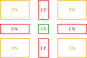
\includegraphics[]{../figures/confusion_matrix_breakout.png}
    \caption{Confusion matrix breakout.}
    \label{fig:confusion_matrix_breakout}
\end{figure}


Each row in the confusion matrix corresponds to an actual class, while each column corresponds to a predicted class This is diagrammed in figure~\ref{fig:confusion_matrix_breakout}. The first row represents non-5 images (the negative class), and the second row represents images classified as 5s (the positive class). The first column of the first row indicates true negatives (TN), while the second column of the first row shows false positives (FP). The second row denotes images of 5s (the positive class): the first column represents false negatives (FN), and the second column displays true positives (TP). A perfect classifier would only have nonzero values along the main diagonal (from top left to bottom right).






\begin{example}
\textbf{Binary Confusion Matrix}

\noindent This example evaluates a binary classifier trained to detect the digit ``5'' using a confusion matrix. The matrix summarizes the number of true positives, true negatives, false positives, and false negatives. It also visualizes specific misclassifications to help interpret where the model fails, such as incorrectly labeling a ``5'' as not a ``5'' (false negative) or misidentifying another digit as a ``5'' (false positive).
\end{example}



\subsubsection{Accuracy, Precision, and Recall}
The confusion matrix provides detailed information, but sometimes a more concise metric is preferred. Before looking into accuracy, let's define it as
\begin{equation}
\text{Accuracy} = \frac{\text{Number of Correct Predictions}}{\text{Total number of Predictions}}
\end{equation}
or
\begin{equation}
\text{Accuracy} = \frac{TP+TN}{TP+TN+FP+FN}.
\end{equation}
While accuracy offers valuable insights, it's essential to consider the number of falsely classified positive and negative predictions, especially within the context of the problem being addressed. For instance, a 99\% accuracy rate might seem satisfactory for predicting credit card fraud. However, what if a false negative indicates a severe virus or cancer? This is why we need to look deeper into the accuracy formula.


%\todo{Look into replacing the verbage of relevant instances and selected instances with True Positives and True Negatives.}
This is where precision and recall come into play. For this, we will need a definitions of instances
\begin{equation}
\text{Selected instances} = TP + FP
\end{equation}
and
\begin{equation}
\text{Relevant instances} = TP + FN
\end{equation}
which are visualized in figure~\ref{fig:piechart_TP_vs_FP}. With these definitions in mind in mind, let's define precision as
\begin{equation}
\text{Precision} = \frac{\text{selected relevant instances}}{\text{selected instances}},
\end{equation}
or,
\begin{equation}
\text{Precision} = \frac{TP}{TP + FP}.
\end{equation}
One way to achieve perfect precision is to make only one positive prediction and ensure it's correct (precision = 1/1 = 100\%). However, this approach would be impractical as it would ignore most positive instances. Recall complements precision by considering all relevant results, both true positives and false negatives. Recall, also known as sensitivity or true positive rate (TPR), is the ratio of positive instances correctly detected by the classifier. We can define recall as
\begin{equation}
\text{Recall} = \frac{\text{selected relevant instances}}{\text{relevant instances}},
\end{equation}
or,
\begin{equation}
\text{Recall} = \frac{TP}{TP + FN}.
\end{equation}

While the definition of accuracy, precision, and recall may not be immediately intuitive, a visualizations such as that shown in figure~\ref{fig:piechart_TP_vs_FP} can help clarify them.

\begin{figure}[H]
    \centering
    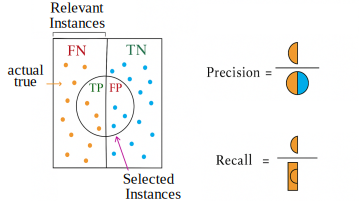
\includegraphics[]{../figures/piechart_TP_vs_FP.png}
    \caption{Visual representation of relevant instances, showing their relation to True Positives (TP) and False Positives (FP). }
    \label{fig:piechart_TP_vs_FP}
\end{figure}


To balance precision and recall, we often use the F1 score, which is the harmonic mean of precision and recall. The F1 score favors classifiers with similar precision and recall, computed as
\begin{equation}
F_1 = 2 \times \frac { \text{precision} \times \text{recall}}{\text{precision} + \text{recall}} = \frac{TP}{TP + \frac{FN + FP}{2}}.
\end{equation}
However, optimizing both precision and recall simultaneously is challenging due to the precision/recall tradeoff. 

Figure~\ref{fig:decision_threshold} illustrates the tradeoffs when adjusting the decision threshold in a Regularized Linear Classifier. By adjusting the classification threshold, we can control the balance between precision and recall. Lowering the threshold increases recall but reduces precision, and vice versa. 
% \todo{add an example on how to adjust the threshold in training.}


\begin{figure}[H]
    \centering
    \includegraphics[]{../figures/decision_threshold.png}
    \caption{Visualization changing thresholds on the classification of digits in a ``5-detector'' and the resulting change in precision and recall.}
    \label{fig:decision_threshold}
\end{figure}

To determine the optimal threshold, it's helpful to plot precision and recall against the threshold values. By default, the classifier in scikit-learn uses a threshold of zero, but this can be adjusted as needed. As illustrated in Figure~\ref{fig:F1_score_plot}, it's relatively straightforward to develop a classifier with nearly any desired precision: simply adjust the threshold to a sufficiently high value. However, it's important to bear in mind that a high-precision classifier may not be very practical if its recall is too low. 




\begin{figure}[H]
    \centering
    \includegraphics[width=6.5in]{../figures/F1_score_plot.png}
    \caption{Visualization of the precision, recall, and F1 score as a function of changing a threshold value. }
    \label{fig:F1_score_plot}
\end{figure}





Figure~\ref{fig:precision_vs_recall} reports a precision vs recall curve that is obtained by changing the threshold of the trained model. At the leftmost part of the precision-recall curve (low recall), precision is highest because the model makes very few positive predictions, and those are likely true positives. As recall increases, the model starts predicting more positives, including more false positives, which reduces precision. The shape of the curve is also important; a steep drop-off indicates that the addition of false positives happens rapidly with increasing recall, whereas a more gradual decline suggests a better balance between precision and recall.

		\begin{figure}[H]
			\centering
			\includegraphics[width=6in]{../figures/precision_recall_curve}
			\caption{The relationship between precision vs recall for a changing threshold value.}
			\label{fig:precision_vs_recall}
		\end{figure}

By analyzing the curve, one can choose a threshold that balances precision and recall according to the specific needs of the application. For instance, in medical diagnosis, high recall is crucial to ensure no cases are missed, even if precision is lower. Additionally, the area under the precision-recall curve (AUC-PR) can be used to compare models. A higher area indicates a model with better performance across all thresholds.

\begin{example}
\textbf{Accuracy, Precision, and Recall}

\noindent This example computes and compares three key classification metrics (accuracy, precision, and recall) for a linear classifier trained to detect the digit ``5'' in the MNIST dataset. It shows both manual and \texttt{sklearn}-based calculations, introduces the F1 score, and visualizes how precision and recall vary with the classification threshold using a precision-recall curve.
\end{example}


\subsection{$k$-fold Cross-validation}
As you've likely observed, training your SGD classifier doesn't always yield consistent results in terms of model performance; hence the ``stochastic'' in stochastic gradient descent. One approach to obtaining a solution closer to the global minimum is to allow the gradient descent algorithm to iterate over more epochs. However, this poses a challenge as it's highly time-consuming and may lead to overfitting the model. Moreover, the variability in model performance makes it difficult to gauge the model's effectiveness.

\begin{figure}[H]
    \centering
    \includegraphics[width=6.5in]{../figures/k-fold_cross-validation_trials}
    \caption{Performance metrics for 500 5-detectors trained either with full data or through $k$-fold cross-validation with 3 folds.}
    \label{fig:k-fold_cross-validation_trials}
\end{figure}

$k$-fold cross-validation offers a more rigorous method for evaluating your algorithm's performance. For instance, consider Figure~\ref{fig:k-fold_cross-validation_trials}, which depicts the performance metrics for 500 classification models trained as 5-detectors. Noticeably, the results obtained using $k$-fold cross-validation exhibit significantly less variability compared to training the classifier on the full dataset. In $k$-fold cross-validation, the training set is divided into smaller subsets for training and validation. The model is trained on these subsets and evaluated on the validation sets. Figure~\ref{fig:grid_search_cross_validation} provides a graphical representation of this technique.

\begin{figure}[H]
    \centering
    \includegraphics[]{../figures/grid_search_cross_validation.png}
    \caption{Illustration of how $k$-fold cross-validation operates.}
    \label{fig:grid_search_cross_validation}
\end{figure}

Of course, Scikit-Learn provides a cross-validation feature, known as \texttt{sk.model\_selection.\allowbreak cross\_val\_score}. This function conducts $k$-fold cross-validation by randomly partitioning the training set into distinct folds. Each fold is used for validation while the rest are used for training the SGD classifier. The reported performance metrics are averaged across all folds. It's important to note that by partitioning the data into folds, the number of samples available for learning is limited, which may result in peculiar classifiers with unusually high or low error rates. Despite being more computationally expensive, this approach effectively utilizes all the data for training and validation.





\begin{example}
\textbf{$k$-fold Cross-Validation}
 
\noindent This example trains a binary classifier to detect the digit ``5'' from the MNIST dataset using Stochastic Gradient Descent (SGD). It first demonstrates how model performance can vary when trained multiple times on the same dataset. Then, by applying $k$-fold cross-validation using \texttt{sk.model\_selection.cross\_val\_predict}, it shows how splitting the data into $k$ subsets helps reduce this variation and provides a more reliable estimate of accuracy, precision, and recall.
\end{example}

\subsection{Multiclass Classification}
Previously, we explored binary classifiers, which distinguish between two classes. Now, we'll explore the use of multiclass classifiers (also known as multinomial classifiers), which can discern between more than two classes. The simplest approach to multiclass classification involves multiple iterations of a binary classifier. There are two primary strategies for achieving this, both of which are considered in the context of the MNIST database challenge:

\begin{itemize}
\item \textbf{One-versus-Rest (OvR)}: This strategy involves creating a system capable of classifying digit images into 10 classes (from 0 to 9) by training 10 binary classifiers, one for each digit (e.g., a 0-detector, a 1-detector, etc.). When classifying an image, the decision score from each classifier is obtained, and the class with the highest score is selected. While sometimes referred to as One-Versus-All (OvA), this term is slightly misleading as it does not involve comparisons against the same class.
\item \textbf{One-versus-one (OvO)}: This approach trains a binary classifier for every pair of digits, such as one for distinguishing between 0s and 1s, another for distinguishing between 0s and 5s, and so forth. If there are $N$ classes, $N \times (N - 1) / 2$ classifiers need to be trained. For the MNIST problem, this translates to training 45 binary classifiers. During classification, the image is evaluated against all 45 classifiers, and the class with the most victories is selected. The primary advantage of OvO is that each classifier only needs to be trained on the relevant portion of the training set for the two classes it distinguishes, which is beneficial for algorithms that scale poorly.
\end{itemize}

\begin{figure}[H]
    \centering
    \includegraphics[width=3.5in]{../figures/one_vs_rest}
    \caption{One-versus-Rest (OvR) classifier for a multi-class dataset.}
    \label{fig:one_vs_rest}
\end{figure}

\begin{figure}[H]
    \centering
    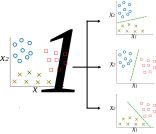
\includegraphics[width=3.5in]{../figures/one_vs_one}
    \caption{One-versus-one (OvO) classifier for a multi-class dataset.}
    \label{fig:one_vs_one}
\end{figure}

Certain algorithms, such as Support Vector Machine classifiers, suffer from scalability issues with larger training sets. Algorithms that do not scale well with large datasets often resort to the OvO approach because training many small classifiers is computationally cheaper than fitting a handful of models on the full data. For most binary classifiers the OvR strategy is the norm. Some methods (including Random Forests and na\"{\i}ve Bayes) support multiclass problems natively and therefore require neither reduction strategy.

\begin{example}
\textbf{Multiclass Regularized Linear Classifier}

\noindent This example extends the use of \texttt{SGDClassifier} to multiclass classification on the MNIST dataset. It compares three approaches: One-vs-Rest (OvR), One-vs-One (OvO), and Scikit-Learn's default automatic strategy. Each method trains multiple binary classifiers to distinguish between the 10 digit classes.
\end{example}



\subsection{Performance Measures for Multiclass Classification}


Assessing a multiclass classifier often poses more challenges compared to evaluating a binary classifier. Nonetheless, many of the principles and methodologies utilized in evaluating binary classifiers can be seamlessly applied to multiclass classifiers as well.


\subsubsection{Confusion Matrix}



%First, you can look at the confusion matrix. You need to make predictions using the \texttt{cross\_val\_predict()} function, then call the \texttt{confusion\_matrix()} function, just like you did earlier:

First, examine the confusion matrix. To do this, generate predictions using the \texttt{cross\_val\_\allowbreak predict()} function, followed by calling the \texttt{confusion\_matrix()} function, similar to your previous steps. The confusion matrix in figure~\ref{fig:digit_confusion_matrix} appears satisfactory, with most images located on the main diagonal, indicating correct classification. However, the 5s appear slightly darker than other digits, suggesting fewer instances of 5s in the dataset or inferior performance of the classifier on 5s. Further investigation confirms both scenarios.




\begin{figure}[H]
    \centering
    \includegraphics[width=4.0in]{../figures/digit_confusion_matrix.png}
    \caption{Confusion matrix for the MNIST data set solved using a one-vs-one classifier with Stochastic Gradient Descent and a $k$-fold of 3.}
    \label{fig:digit_confusion_matrix}
\end{figure}



To turn figure~\ref{fig:digit_confusion_matrix} into a figure that highlights the mistakes, first normalize each entry of the confusion matrix by the number of images in its true class so you compare error rates rather than raw counts that would overweight frequent classes. Then set the diagonal cells to \texttt{NaN} so only the off-diagonal errors remain visible, and plot the resulting matrix. The resulting figure~\ref{fig:digit_confusion_matrix_2} more clearly highlights the errors in the confusion matrix.


\begin{figure}[H]
    \centering
    \includegraphics[width=4.0in]{../figures/digit_confusion_matrix_error.png}
    \caption{Normalized confusion matrix (similar to figure~\ref{fig:digit_confusion_matrix}) with the diagonal removed to emphasize errors.}
    \label{fig:digit_confusion_matrix_2}
\end{figure}

The refined plot facilitates a clear understanding of the classifier's error patterns. Rows represent actual classes, while columns depict predicted classes. Columns corresponding to classes 8 and 9 exhibit brightness, indicating numerous misclassifications as 8s or 9s. Likewise, rows for classes 8 and 9 also appear bright, signifying frequent confusion between 8s, 9s, and other digits. Conversely, some rows, like row 1, display darkness, indicating accurate classification of most 1s (with few exceptions confused with 8s). Notably, errors are asymmetric; for instance, more 5s are misclassified as 8s than vice versa.

Analyzing the confusion matrix provides valuable insights for classifier enhancement. In this case, efforts should concentrate on improving the classification of 8s and 9s, along with addressing the specific 3/5 confusion. Potential strategies include gathering more training data for these digits, devising new features (e.g., counting closed loops), or preprocessing images to emphasize distinguishing patterns (e.g., using Scikit-Image, Pillow, or OpenCV).



\subsubsection{Analyzing Individual Errors}

Analyzing individual errors provides valuable insights into the classifier's behavior and reasons for its failures.

\begin{figure}[H]
    \centering
    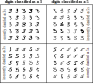
\includegraphics[]{../figures/3s_and_5s.png}
    \caption{Confusion matrix showing digits classified as 3s and 5s for the same classifier used to obtain the results shown in figure~\ref{fig:digit_confusion_matrix}.}
    \label{fig:3s_and_5s}
\end{figure}

The left half of figure~\ref{fig:3s_and_5s} contains the blocks for images the classifier labelled as 3, while the right half shows those it labelled as 5. A few misclassified digits are so poorly written that even a human might hesitate, yet many errors look quite clear. Remember that a regularised linear classifier assigns a single weight to every pixel for each class and then sums the weighted pixel intensities to score each class. 

Because just a handful of pixels separate a 3 from a 5, a linear classifier often confuses the two. Their main distinction is the small stroke that joins the top bar to the bottom curve; even a slight shift or rotation of this junction can flip the prediction. The linear model is therefore very sensitive to translations and rotations. Pre-processing the images to center the digits and correct their orientation should lessen the 3-5 confusion and improve performance across the board.
5 

A non-linear model can learn more complex patterns by applying transformations (such as kernel mappings), effectively giving different relative importance to various parts of the image, and would therefore be better equipped to  capture more intricate pixel patterns and more effectively separate these digits.






\begin{example}
\textbf{Multiclass Confusion Matrix}

\noindent This example uses a One-vs-One classifier trained with Stochastic Gradient Descent to evaluate multiclass classification performance on the MNIST dataset. It constructs a confusion matrix using 3-fold cross-validation and visualizes both the raw classification counts and the normalized error rates, helping identify which digits are most commonly misclassified.
\end{example}

\pagebreak
\includepdf[pages=-, width= 0.95\textwidth, pagecommand = {\subsection{Examples} \subsubsection*{Example 3.1}\vspace{0.5em}}]{../code/example_3.1_load_MNIST.pdf}

\includepdf[pages=1, width= 0.95\textwidth, pagecommand = {\subsubsection*{Example 3.2}\vspace{0.5em}}]{../code/example_3.2_MNIST_SGD.pdf}
\includepdf[pages=2, width= 0.95\textwidth, pagecommand = {\vspace{0.5em}}]{../code/example_3.2_MNIST_SGD.pdf}

\includepdf[pages=1, width= 0.95\textwidth, pagecommand = {\subsubsection*{Example 3.3}\vspace{0.5em}}]{../code/example_3.3_confusion_matirx.pdf}
\includepdf[pages=2, width= 0.95\textwidth, pagecommand = {\vspace{0.5em}}]{../code/example_3.3_confusion_matirx.pdf}

\includepdf[pages=1, width= 0.95\textwidth, pagecommand = {\subsubsection*{Example 3.4}\vspace{0.5em}}]{../code/example_3.4_precision_recall_accuracy.pdf}
\includepdf[pages=2, width= 0.95\textwidth, pagecommand = {\vspace{0.5em}}]{../code/example_3.4_precision_recall_accuracy.pdf}

\includepdf[pages=1, width= 0.95\textwidth, pagecommand = {\subsubsection*{Example 3.5}\vspace{0.5em}}]{../code/example_3.5_k-fold_cross-validation.pdf}
\includepdf[pages=2, width= 0.95\textwidth, pagecommand = {\vspace{0.5em}}]{../code/example_3.5_k-fold_cross-validation.pdf}

\includepdf[pages=-, width= 0.95\textwidth, pagecommand = {\subsubsection*{Example 3.6}\vspace{0.5em}}]{../code/example_3.6_Multiclass_SDG.pdf}

\includepdf[pages=-, width= 0.95\textwidth, pagecommand = {\subsubsection*{Example 3.7}\vspace{0.5em}}]{../code/example_3.7_multiclass_confusion_matrix.pdf}

\end{document}

